\section{Zielsetzung}
\label{sec:Zielsetzung}
Diodenaser sind von zentraler Bedeutung in der Physik, da mit ihrem starken Output von kohärenten
Licht innerhalb eines schmalen Frequenzsprektrums sehr gut atomare Strukturen bzw. Quantensysteme
untersucht werden können. Außerdem können die Laser auf eine bestimmte Wellenlänge eingestellt werden, 
wodurch sie sich optimal auf das zu untersuchende System anpassen lassen.
In diesem Versuch soll die Funktionsweise eines Diodenlasers näher untersucht werden, indem die
Fluoreszenz von Rubidium nachgewiesen wird. Dafür müssen die verschiedenen Laserparamter so justiert werden,
dass die für Rubidium benötigte Wellenlänge erzeugt wird.

\section{Theorie}
\label{sec:Theorie}

Bevor der Aufbau eines Diodenlaser erläutert wird, folgen zuerst die physikalischen Grundlagen von Photonenemmission
sowie Halbleitern und Dioden, da diese essentiell für das Verständniss der Funktionsweise eines Diodenlasers sind.

\subsection{Absorption und Emmission in Zustandssystemen}

In quantenmechanischen Systemen liegen diskrete Energieniveaus vor, das einfachste Beispiel hierfür ist ein Zweizustandssystem
mit einer Grundzustandsenergie $E_1$ und einem angeregten Zustand mit der Energie $E_2$. Um in einen
angeregten Zustand zu wechseln, kann ein Teilchen ein Photon absorbieren, falls die Energie des Photons genau der
Energiedifferenz der Niveaus entspricht:
\begin{equation}
    \notag
    E_{\text{ph}} = E_2 - E_1 = h \omega
\end{equation}
Umgekehrt muss ein Photon emmitiert werden, wenn das Teilchen wieder auf den Grundzustand wechselt.
Die Emmission des Photons kann zufällig erfolgen (spontane Emmission), oder durch ein anderes Photon
ausgelöst werden (stimulierte Emmission). Bei der stimulierten Emmission wird zusätzlich zu dem Photon,
dass die Emmission ausgelöst hat, ein zweites Photon erzeugt. Dieses Photon ist hinsichtlich aller seiner
Eigenschaften wie Frequenz, Polarisation und Phase identisch zum ersten Photon. Somit ist leicht
ersichtlich, warum dieser Vorgang in Lasern ausgenutzt wird. Findet er oft genug statt, so wird eine
ganz spezifische Wellenlänge an Licht starkt verstärkt, die dann zum Experimentieren genutzt werden kann.

Damit die stimulierte Emmission im Vergleich zur spontanen Emmission überwiegen kann, muss der energetisch
höhere Zustand häufiger besetzt sein als der niedrige, dies wird auch als Besetzungsinversion bezeichnet.
In dem zuvor beschriebenen Zweizustandssystem lässt sich dies nicht realisieren. Da die Übergangwahrscheinlichkeit
von $E_1$ zu $E_2$ genau so groß ist wie von $E_2$ zu $E_1$, kann höchstens
eine Gleichbesetzung erreicht werden.

Sobald ein oder mehrere weitere Zustände hinzugefügt werden, kann dieser Effekt jedoch auftreten.
In \autoref{fig:Besetzungsinversion} ist der simpelste Fall, also ein Dreizustandssystem, abgebildet.
\begin{figure}[H]
    \centering
    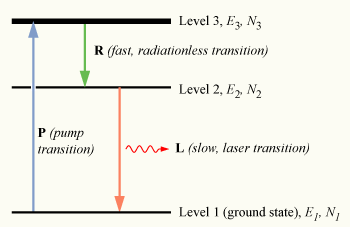
\includegraphics[height=6cm]{content/pics/besetzungsinversion.png}
    \caption{Skizze eines Dreizustandssystems und den möglichen Übergängen. \cite{Besetzungsinversion}}
    \label{fig:Besetzungsinversion}
\end{figure}
Es existiert ein drittes Energieniveau $E_3$, in dass die Teilchen durch die eingehenden Photonen gepumpt werden.
Dannach fallen sie sehr schnell ohne Emmission eines Photons in den mittleren Zustand $E_2$. Von dort aus kann
die zuvor beschriebene, langsamere stimulierte Emmission stattfinden. Alle Teilchen die im Grundzustand landen,
werden durch die anderen Photonen direkt wieder in den höchsten Zustand versetzt. Somit verweilen die meisten
Teilchen im mittleren Zustand $E_2$ und die zuvor beschriebene Besetzungsinversion wurde erreicht.

\subsection{Halbleiter und Dioden}

\subsection{Aufbau eines Diodenlasers und Justierung}

\begin{figure}[H]
    \centering
    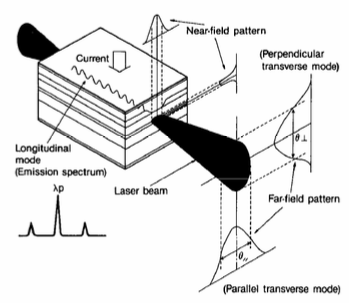
\includegraphics[height=8cm]{content/pics/laser.png}
    \caption{Laserskizze. \cite{V60}}
    \label{fig:laser}
\end{figure}

\begin{figure}[H]
    \centering
    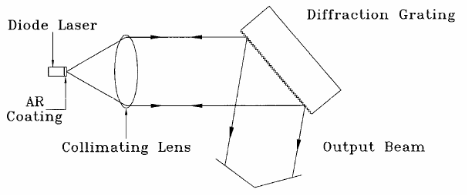
\includegraphics[height=5cm]{content/pics/graiting.png}
    \caption{graiting. \cite{V60}}
    \label{fig:graiting}
\end{figure}

\subsection{Absorptionsspektrum von Rubidium}

\begin{figure}[H]
    \centering
    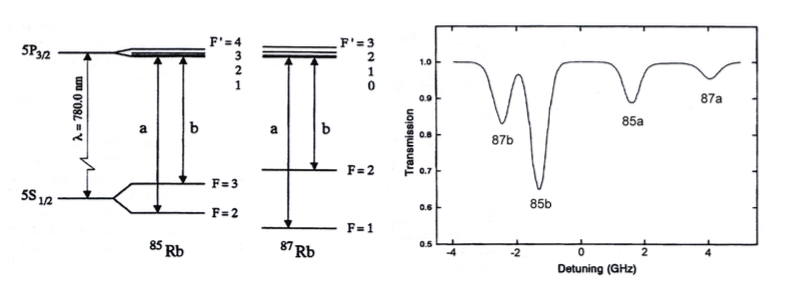
\includegraphics[height=5cm]{content/pics/Rubidium.png}
    \caption{Rubidium. \cite{V60}}
    \label{fig:rubidium}
\end{figure}

